\begin{section}{Preguntas}

A continuación pasamos a responder algunas de las preguntas enunciadas en el trabajo práctico.
\begin{itemize}
	\item ¿Depende la forma de la curva de la elección de la parametrización?
	
		Como vimos en los gráficos de la sección resultados, la elección de la parametrización está completamente ligada a la forma de la curva. Como ejemplo de esto podemos hacer referencia a los gráficos \ref{fig:5p}, \ref{fig:5p_r} y \ref{fig:5p_u}. Si bien todas las parametrizaciones comparten ciertos puntos (por ejemplo los mismos puntos de control), la forma en que aproximan a la curva es distinta.

	\item ¿Cambia la forma de la curva si en lugar de deformar la curva conservando la parametrización o el programa la recalcula al mover el punto?

	Para poder responder esta pregunta modificamos el código en una carpeta aparte para poder recalcular la parametrización y graficamos los resultados en tres archivos distintos, donde en cada uno de ellos se utilizó sólo una parametrización. La curva es igual para los tres graficos.
	Se presentan en el siguiente orden los gráficos, utilizando la parametrización uniforme , la centrípeta y por último por longitud de cuerda.
	
	\begin{figure}[H]
		  \centering
			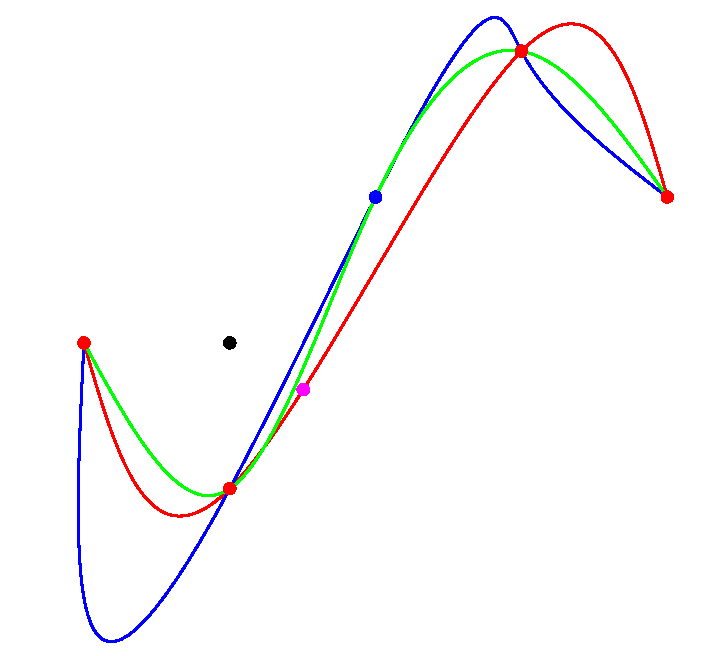
\includegraphics[width=14cm]{graficos/paramVSreparamUniform.pdf}
		  \caption{Cambio de parametrización (Uniforme)}
		  \label{fig:paramChangeUniform}
	\end{figure}
	
	\begin{figure}[H]
		  \centering
			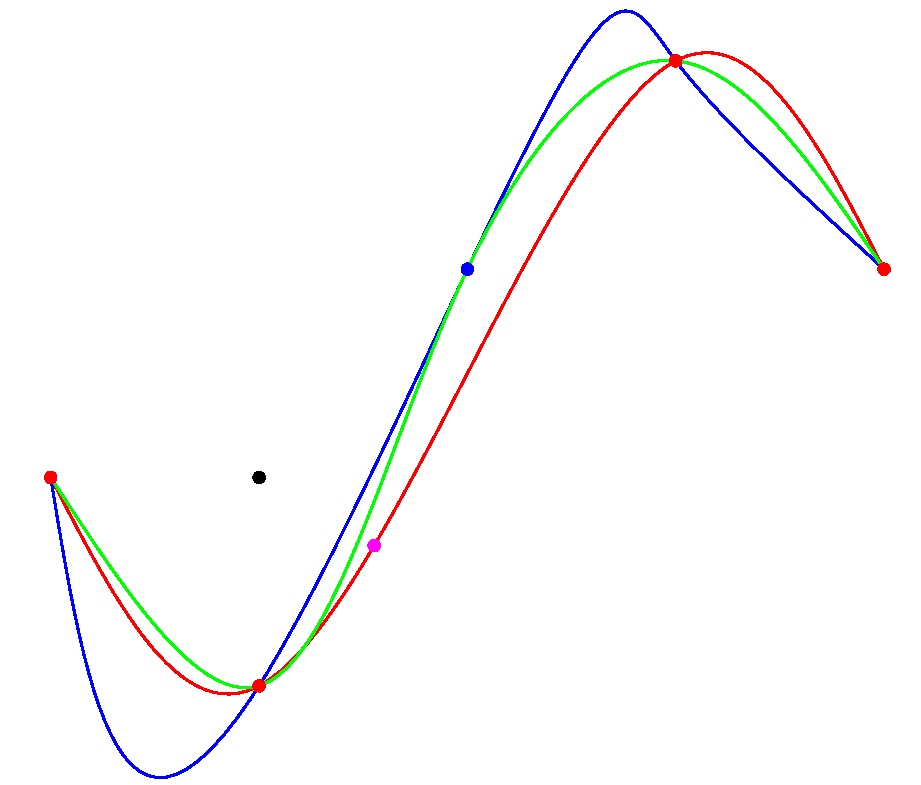
\includegraphics[width=14cm]{graficos/paramVSreparamCentripetal.pdf}
		  \caption{Cambio de parametrización (Centrípeta)}
		  \label{fig:paramChangeCentripetal}
	\end{figure}

	\begin{figure}[H]
		  \centering
			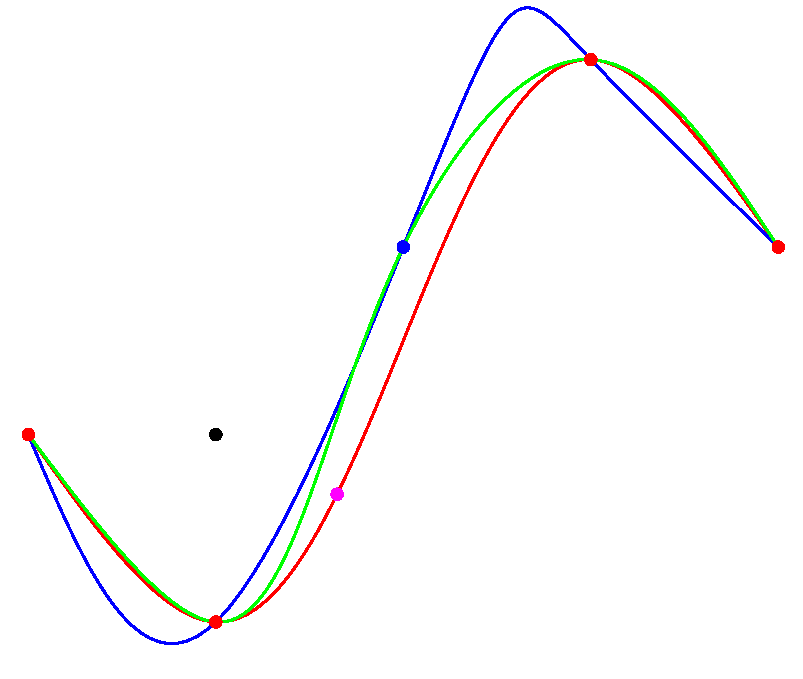
\includegraphics[width=14cm]{graficos/paramVSreparamChord.pdf}
		  \caption{Cambio de parametrización (Longitud de cuerda)}
		  \label{fig:paramChangeCHLength}
	\end{figure}
	\VSP

\end{itemize}	



\end{section}
